\newpage
\section{Image Compression Example [Optional]}
\newthought{The Fourier series can be generalized to two-dimensional
  signals $I:\mathbb{R}^2 \rightarrow \mathbb{C}$}. The two-dimensional 
  Fourier series is often used in image processing and image
compression.

The Fourier series representation for a two-dimensional periodic
function with period $T_x$ in the $x$ direction and $T_y$ in the $y$
direction is:
\begin{equation}
I(x,y) = \sum_{n,m \in \mathbb{Z}} c_{n,m} e^{i \frac{2\pi}{T_x}nx} e^{i \frac{2\pi}{T_y}my} \,\,.
\end{equation}
The analysis procedure to obtain the coefficients $c_{n,m}\in \mathbb{C}$ is:
\begin{equation}
c_{n,m} = \frac{1}{T_x T_y}\int_{0}^{T_x}\int_0^{T_y} I(x,y) e^{-i \frac{2\pi}{T_x}nx} e^{-i \frac{2\pi}{T_y}my}dx dy \,\,.
\label{eq:2d_analysis}
\end{equation}
Many of the familiar results for 1d signals, such as the time shifting
property, or differentiation, can be extended to 2d or higher
dimensional periodic functions. 
%All of the results regarding differentiation and ``time shifting'' can
%be generalized to multiple dimensions. For example, time shift in two
%dimensions $I(x+\tau_x,y+\tau_y)$ is equivalent to translation in $x$
%and $y$, and this operation can be applied directly on the constants
%$c_{n,m}$.


\newthought{In this programming example I'll briefly demonstrate to 
you the concept of spectral image compression}.  It is possible to
extend the idea of compression of a one dimensional signal, as
demonstrated in the audio compression example, by only storing strong
frequency components in 2D images. This is essentially the idea
behind the JPEG image compression algorithm.  The Python code in
Listing \ref{lst:image_compression} demonstrates image compression and
produces the image shown in Figure \ref{fig:image_compression}. The
program uses the 2D discrete-Fourier transform function,
\verb|numpy.fft.fft2|, to calculate the phases and amplitudes of the
spectral components, $c_{n,m}$, of the image. It then uses the 2D
inverse discrete Fourier transform to FFT synthesize an image from
only 5\% of the spectral components. The output of the image
compression example is shown in Figure \ref{fig:image_compression}. It
shows the original and compressed image that is formed using a sparse
Fourier series representation of the image. The magnitudes of the
spectral components for the compressed and original image are also
shown.

\begin{figure}
\begin{center}
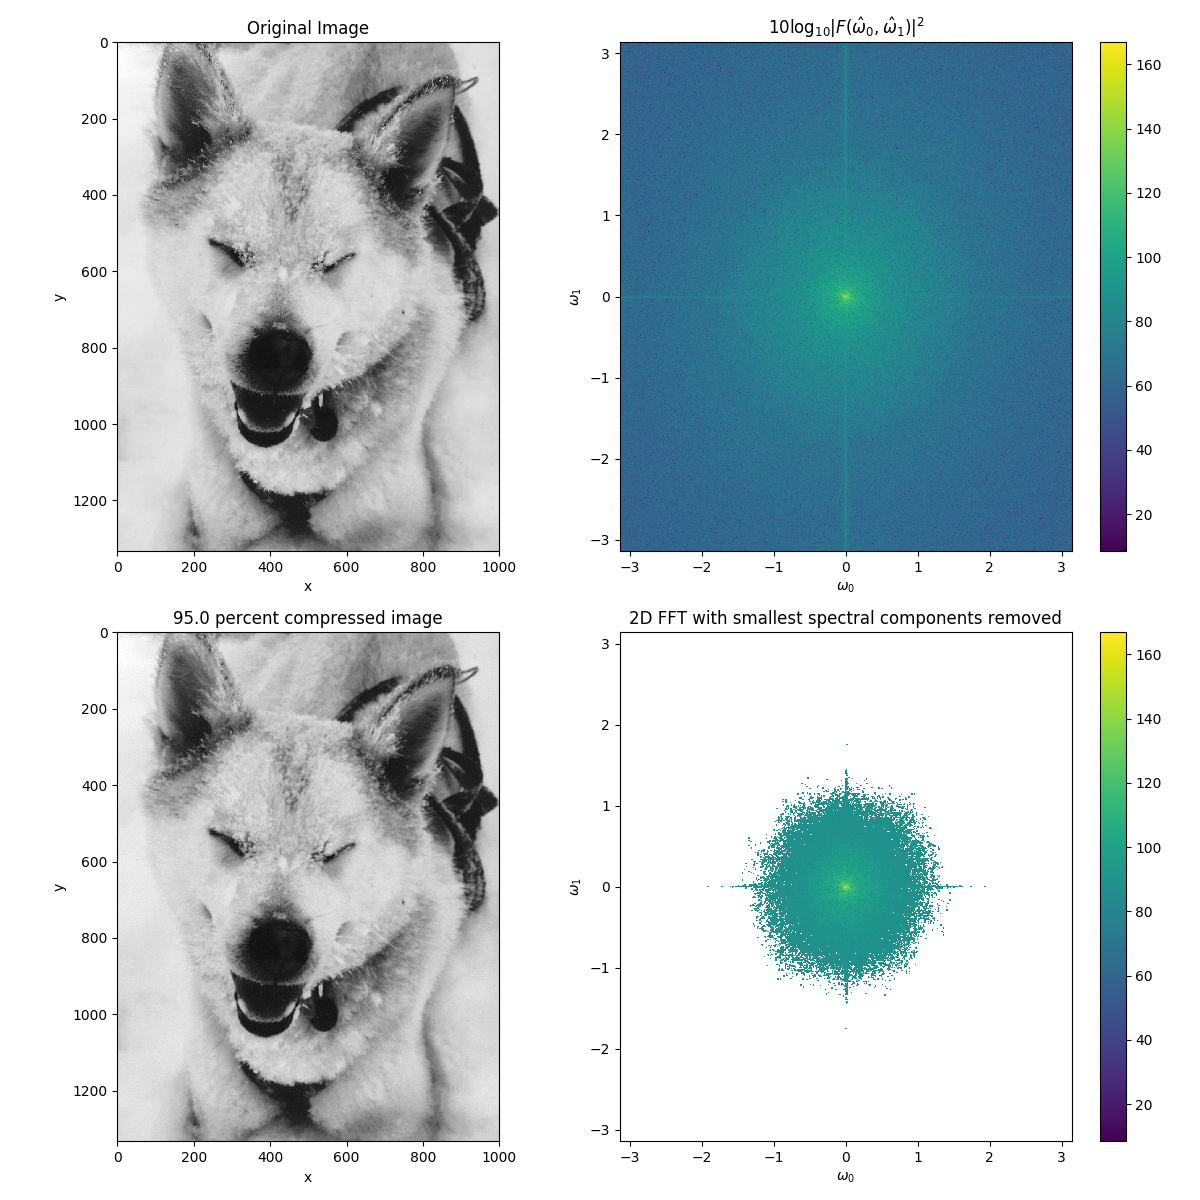
\includegraphics[width=0.93\textwidth]{Applications/figures/image_compression.png}
\end{center}
\caption{Image compression example. Top left: original image, Top
  right, the magnitude squared of the spectral components in dB
  scale. Bottom left: compressed image formed using only 5\% of the
  strongest spectral components. Bottom right: the spectral magnitude
  squared of the spectral components used to form the image on the
  bottom left.}
\label{fig:image_compression}
\end{figure}

The same words of warning that I gave with the audio compression
example apply to this program example. If you are only beginning with
Python, you may have a hard time with understanding this program. For now, you can think of the 2D FFT and inverse FFT as an analysis and synthesis step for a 2D
periodic function. But don't let a warning or lack of experience
prevent you from exploring!

\lstinputlisting[language=Python,caption={\texttt{011\_image\_compression/image\_compression.py}},label=lst:image_compression]{code/011_image_compression/image_compression.py}
